In questa sezione si presentano diversi algoritmi che operano sulle Stream
\begin{itemize}
    \item Stima delle frequenze di elementi (Sampling e CountMin)
    \item Filtro di Stream (Bloom filters)
    \item Conteggio del numero di elementi diversi (Flajolet-Martin)
    \item Stima dei momenti (Algoritmo AMS)
\end{itemize}

\subsection{Stima delle frequenze}
Data una Stream $x_1,\dots,x_m$ di interi con $x_i \in [n]$ e per ogni elemento $y \in [n]$ si definisce la frequenza di $y$ come il numero di volte in cui $y$ appare nella Stream
\[
    f_y = |\{i: x_i = y\}|
\]
\subsubsection{Sampling}
La prima soluzione fa uso del \emph{Sampling}, assumendo di conoscere la lunghezza della stream $(m)$, se così non fosse si fa uso del \emph{Reservoir Sampling} \ref{reservoir}, si scelgono $j_1,\dots,j_q \in_u [1,m]$ con $q$ valore determinato in un secondo momento. Durante la Stream vengono salvati gli elementi $x_{j_1},\dots,x_{j_q}$ creando così uno \emph{sketch}. Si definisce l'indicatore booleano $\mathbb{I}_{x=y}$
\[
    \mathbb{I}_{x=y} = 
    \begin{cases*}
        1 \text{ se } x = y\\
        0 \text{ altrimenti}     
    \end{cases*}
\]
\begin{lemma}
    Per ogni dati $y$ e $x_j$
    \[
        \E{\mathbb{I}_{x_{j}=y}} = \frac{f_y}{m}
    \]
\end{lemma}
\begin{proof}
    Ogni elemento della Stream ha probabilità $\frac{1}{m}$ di essere scelto come $x_{jk}$ ogni $y$ ha $f_y$ occorrenze nella Stream.
\end{proof}

Ora è possibile affermare che
\begin{equation}
    \label{eq:1}
    \E{\sum_{k=1}^{q}{\mathbb{I}_{{x}_{jk} = y}}} = q \cdot \frac{f_y}{m} = \frac{q}{m}\cdot f_y
\end{equation}
È possibile calcolare lo stimatore $\tilde{f_y} = \frac{m}{q} \cdot \sum_{k=1}^{q}{\mathbb{I}_{{x}_{jk} = y}}$ facendo uso dello \emph{sketch}, inoltre, per (\ref{eq:1}), si ha uno stimatore \emph{senza bias}.

In altre parole $\tilde{f_y}$ è il numero di occorrenze di $y$ nel \emph{sample} scalato per un fattore $\frac{m}{q}$, banalmente si ottiene:
\begin{lemma}
    \[
        \E{\tilde{f_y}} = f_y
    \]
\end{lemma}
\begin{proof}
    \[
        \frac{m}{q}\E{\sum_{k=1}^{q}{\mathbb{I}_{{x}_{jk} = y}}} = \frac{m}{q}\cdot{\frac{q}{m}\cdot f_y} = f_y
        \]
        
\end{proof}
applicando il Chernoff bound
\begin{align}
    \Pr[|\tilde{f_y} - f_y| > \varepsilon m] &= \Pr\left[ \frac{q}{m} |\tilde{f_y} - f_y| > \varepsilon q \right] = \\
    &= \Pr\left[ \left|\sum_{k=1}^{q}{\mathbb{I}_{{x}_{jk} = y}} - \E{\sum_{k=1}^{q}{\mathbb{I}_{{x}_{jk} = y}}}\right| > \varepsilon q \right]\\
    %&\Pr\left[ \left|\sum_{k=1}^{q}{\mathbb{I}_{{x}_{jk} = y}} - \E{\sum_{k=1}^{q}{\mathbb{I}_{{x}_{jk} = y}}}\right| > \varepsilon q \right] < \\
    \substack{\text{Per il}\\ \text{Chernoff Bound}}&< 2 \exp\left(-\frac{(\varepsilon q)^2}{2q}\right) = 2 \exp\left(-\frac{\varepsilon^2 q}{2}\right)
\end{align}
Si vuole $(1) < \delta$ per cui si deve ottenere $q$ tale che $q > \varepsilon^{-2}\log\left(\frac{2}{\delta}\right)$

\begin{theorem}
    Dato un fattore di approssimazione $\varepsilon$ e un parametro di confidenza $\delta$, in una qualsiasi Stream di $m$ elementi e per ogni elemento $y$ l'algoritmo restituisce uno stimatore \emph{unbiased} $\tilde{f_y}$ tale che $|\tilde{f_y}- f_y| < \varepsilon m$ con probabilità almeno $1- \delta$. La complessità spaziale è $O(\varepsilon^{-2} \log\left(\frac{2}{\delta}\right))$
\end{theorem}

\subsubsection{Algoritmo Min-Sketch}
Il count Min-Sketch è un metodo che utilizza (asintoticamente) meno spazio rispetto al metodo visto in precedenza basato sul \emph{sampling}, inoltre ha un errore del tipo \emph{one-sided}.

\begin{definition}[Count MinSketch]
    Il count MinSketch è una matrice $M \in \mathbb{N}^{t\times s}$ inizializzata a 0. $s \times t$ determina il fattore di errore e la probabilità di successo. A ogni riga $j$ è associata una funzione hash universale $h_j: [1,n] \to [1,s]$ per $j = 1,\dots,t$
\end{definition}

Si definisce l'inserimento di un elemento $x$ nello \emph{sketch}, per ogni $j=1,\dots,t$
\[
    M(j,h_{j}(x)) = M(j,h_{j}(x)) + 1
\]
e la procedura per il calcolo delle stime delle frequenze: $M(j,h_{j}(x))$ è il contatore delle volte che l'elemento $y$ è stato visto. Per la stima delle frequenze si restituisce $\tilde{f_y} = \min\{M(j,h_{j}(x)): j = 1,\dots,y\}$. 

Si nota che si hanno a disposizione $t$ funzioni hash indipendenti, di cui ognuna mappa un elemento della Stream in $s$ slot differenti. Poiché il contatore $M(j,h_{j}(x))$ viene aumentato ogni volta che l'elemento $y$ viene visto nella Stream. Si ha quindi 

\begin{enumerate}
    \item per ogni $y \in [n]$, $M(j,h_{j}(x)) \geq f_y$ non fornisce mai una sottostima
    \item per ogni $z \in [n]$, con $z \neq y$ tali che $h_j(z) = h_j(y)$ (ovvero due elementi per cui si ha una collisione) si ha che $M(j,h_{j}(x)) = f_y +f_z$
\end{enumerate}

Come studiato, l' hashing universale minimizza il numero di collisioni, per cui lo stimatore $\tilde{f_y} = \min\{M(j,h_{j}(x)): j = 1,\dots,y\}$ sbaglia solo se avviene una collisione in tutte le funzioni hash $j = 1,\dots,t$. 

Si cerca di stimare la probabilità $\Pr[M(j,h_{j}(x)) > f_y + \varepsilon m]$ per $\varepsilon > 0$, a tale scopo si definisce la variabile aleatoria $\mathbb{I}(j,x,y)$ come segue 
\[
    \mathbb{I}(j,x,y) = 
    \begin{cases*}
        1 \text{ se } h_j(x) = h_j(y)\\
        0 \text{ altrimenti}
    \end{cases*}
\]

Sia $S = \{x_1,\dots,x_m\}$ l'insieme degli elementi distinti nella Stream, si calcola il valore atteso di $M(j,h_{j}(y))$

\begin{align*}
    \E{M(j,h_{j}(y))} = f_y + \E{\sum_{x \neq y} f_x \mathbb{I}(j,x,y)} = f_y + \sum_{x \neq y} f_x \E{\mathbb{I}(j;x,y)}
\end{align*}
Inoltre poiché $h_j(y)$ fa uso di hashing universale su una tabella di $s$ slot e $\sum_{x \in S}f_x = m$
\begin{align*}
    &f_y + \sum_{\substack{x \in S \\ x \neq y}}f_x \E{\mathbb{I}(j,x,y)} \leq f_y + \sum_{x \neq y}f_x \frac{1}{s}\\
    &= f_y + \frac{1}{s}\sum_{x \neq y}f_x \leq f_y + \frac{m}{s}
\end{align*}
Poiché si fa uso $h_j$ universale $\Pr[h_j(x) = h_j(y)] \leq \frac{1}{s}$, si conclude che $\E{M(j,h_j(y)) - f_y} \leq \frac{m}{s}$, facendo uso della disuguaglianza di Markov
\[
    \Pr[M(j,h_j(y)) -f_y \geq 2 m/s] \leq \frac{1}{2} \text{ e per } \varepsilon > 0 \ \ \frac{2m}{s} = \varepsilon m
\]
\begin{lemma}
    Per ogni $\varepsilon > 0$ per ogni $j = 1,\dots,t$ e scegliendo $s = \frac{2}{\varepsilon}$ si ha 
    \[
        \Pr[M(j,h_j(y)) \geq f_y + \varepsilon m] \leq \frac{1}{2} 
    \]
\end{lemma}

Qual è la probabilità che lo stimatore $\tilde{f_y} > f_y + \varepsilon m$, si ricorda che lo stimatore $\tilde{f_y}$ è definito come il minimo fra tutte le righe, se il minimo supera  $f_y + \varepsilon m$ allora tutte le righe lo superano, e poiché le funzioni hash $h_j$ sono scelte indipendentemente
\[
    \Pr[\tilde{f_y} \geq f_y + \varepsilon m]  \leq \left( \frac{1}{2}\right)^t
\] 
e definendo $\delta = \left( \frac{1}{2}\right)^t$, risolvendo per $t$ si ottiene che per $t = \lceil \log_2(\frac{1}{\delta}) \rceil$ la stima di $\tilde{f_y}$ soddisfa $f_y \leq \tilde{f_y} \leq f_y + \varepsilon m$ con probabilità $\geq 1 - \delta$.

\begin{theorem}
    Scegliendo $\varepsilon > 0$ (errore), e $\delta > 0$ (probabilità di fallimento) per una $s = 2/\varepsilon$ fissata e $t = \log(1\delta)$ il \emph{MinSketch} $M$ usa $O\left( \frac{\log 1/s}{\varepsilon}\right)$ parole di spazio e $f_y \leq \tilde{f_y} \leq f_y + \varepsilon m$ con probabilità $\geq 1 - \delta$. Il tempo di aggiornamento e query è $O(\log(1/\delta))$.
\end{theorem}

\subsection{Filtro delle Stream}
Si parla ora di filtro su Stream: ogni elemento $x$ nella Stream è una tupla $x = <k_1,\dots,k_k>$, in input è data un insieme $S$ di valori ``buoni'' per le tuple aventi una particolare chiave $k$.

\vspace{1em}\noindent
Una soluzione banale consiste nel salvare $S$ in una tabella hash $T$, per ogni elemento $x$ viene calcolata l'hash di $k(x)$, successivamente verificata con la tabella $T$.

Un problema è evidente quando l'insieme $S$ è troppo grande da non poter essere mantenuto interamente in memoria

\subsubsection{Algoritmo First-Cut}
Sia $U = \{ \text{tutti i valori possibili per la chiave $k$} \}$, e $S$ l'insieme di tutti i valori ``buoni'' della chiave $k$ scelta, l'algoritmo si sviluppa ora in 2 fasi

\begin{enumerate}
    \item[Fase 1:]
    Viene creato un array $B[1,n]$ di $n$ bit, inizializzato a 0
    
    Viene scelta una funzione hash $h: U \to [n]$
    
    Per ogni componente $s \in S$ viene calcolato il valore hash $h(s)$
    
    Viene impostato $B[h(s)] = 1$ 
    
    \item[Fase 2:]
    
    Sia $x = <x_1,\dots,x_k>$ un nuovo elemento della Stream
    
    Viene calcolato $h(x_k)$
    
    Se $B[h(x_k)] = 1$ l'elemento $x$ è accettato
\end{enumerate}

Questo metodo permette dei falsi positivi, ma mai dei falsi negativi (\textit{one-sided-error}). Analisi dell'algoritmo 
\begin{theorem}
    Se un elemento è in $S$, allora sicuramente il nel vettore $B$ esiste la posizione corrispondente uguale a 1. Si ha un falso positivo solo nel caso di collisione
\end{theorem}

\vspace{1em}\noindent
Si analizza più nel dettaglio l'algoritmo, per calcolare la probabilità di falsi positivi sia $|S| = m$, $|B| = n$ (ovvero il numero di \emph{bucket}), per qualche elemento $u \in U$ la probabilità di finire in una posizione di $B$ già inizializzata a 1 è esattamente la frazione \emph{ERR} di \emph{bucket} in $B$. Si procede stimando \emph{ERR} con l'esperimento \textit{balls into bins}.
Mandando $m$ palline in $n$ \emph{bucket} con la stessa probabilità per ognuno, qual è la probabilità che un \emph{bucket} riceva almeno una pallina. 

\vspace{1em}
In questo caso i \emph{bucket} sono $0,\dots,n-1$, mentre le palline sono i valori hash $h(k(x))$ degli elementi $S = \{1,2,\dots,m\}$, la probabilità che una pallina finisca in un \emph{bucket} è $\frac{1}{n}$ allora 
\[
    \Pr[\emph{ERR}] = 1 - \left(1-\frac{1}{n}\right)^m \approx 1 - e^{-\frac{m}{n}}
\]
per $m$ molto più piccolo di $n$, $\Pr[\emph{ERR}] \approx \frac{m}{n}$

Si è ottenuto quindi che la frazione dei falsi positivi è proprio $1-e^{-\frac{m}{n}}$

\subsubsection{Filtri di Bloom}
Si consideri $|S| = m$, $|B| = n$ si fa uso di $k$ funzioni hash indipendenti $h_1,\dots,h_k$, si descrive il processo di inizializzazione:
\begin{itemize}
    \item si imposta $B = [0,\dots,0]$
    \item si esegue l'hash degli elementi $s \in S$, facendo uso di ogni funzione hash, $h_i$ $B[h_i(s)]$
\end{itemize}
e il processo di esecuzione
\begin{itemize}
    \item quando viene ricevuto un elemento con chiave $x$
    \item se $B[h_i(x)] = 1$ per $i = 1,\dots,k$ $x$ viene accettato
\end{itemize}

Si procede facendo un'analisi dell'algoritmo, si analizza quindi il numero di \emph{bucket} nel vettore $B$ contenenti \textit{1}, la vengono fatti $k\cdot m$ tentativi per $n$ \emph{bucket}, quindi la frazione di \textit{1} è \[
    1-e^{-\frac{k\cdot m}{n}} \approx \frac{k\cdot m}{n}
\] e poiché le $k$ funzioni hash sono mutualmente indipendenti e $x$ viene accettato se tutti i \emph{bucket} contengono \textit{1}. La probabilità dei falsi positivi è $\left( 1 - e^{-\frac{k\cdot m}{n}}\right)^k$.

\vspace{1em}\noindent
È necessario determinare un valore di $k$ ottimale, in cui la funzione è minima, con l'analisi matematica si ottiene il valore di $k = \frac{n}{m}\log(2)$.

\subsection{Conteggio degli elementi distinti}
Il problema del conteggio consiste nel, data una Stream di elementi scelti da un universo $U$ di dimensione $N$, mantenere un contatore $d$ di elementi distinti visti fino ad ora.

\vspace{1em}
Un approccio banale consiste nel mantenere un insieme di elementi precedentemente visti, attraverso una tabella hash.

Con la limitazione nello spazio se si è disposti ad accettare un margine di errore ma con una probabilità limitata è possibile fare uso dell'approccio di \textit{Flajolet-Martin}.

In cui in una fase preliminare viene scelta una funzione hash $h$ che mappa ognuno degli $N$ elementi di $U$ in almeno $\log_2(N)$ bit 
\[
    h:[N] \to \{0,1\}^s \ \ s\geq \log_2(N)
\]
Per ogni elemento della Stream $a$ sia $r(a) =$ posizione del primo \textit{1} contando dalla destra in $h(a)$,  $R = \max\{r(a)\}$ visto $\forall a$. Il valore stimato $m = 2^R$. 

Si annunciano le proprietà utili dell'algoritmo \textit{FM}: per le occorrenze ripetute dello stesso elemento, il valore stimato $R$ non viene \text{mai} modificato.

Lo \emph{Sketch} $R$ può essere facilmente combinato con altri, avendo gli \emph{Sketch} $R_1,R_2,\dots, R_k$ da differenti Stream, essi possono essere combinati calcolando $\max(R_1,R_2,\dots,R_k)$. Segue una breve dimostrazione del funzionamento del metodo

\begin{proof}
    Si assuma $h: [N] \to \{0,1\}^s$ con $s \geq \log(N)$, poiché $h$ è una funzione hash perfetta
    \begin{itemize}
        \item Per ogni $a$ vale che $\Pr[r(a) \geq r] = \left(\frac{1}{2}\right)^r$
        
        Sia la variabile aleatoria $X_r = \begin{cases*}
            1 \text{ se $\exists \bar{a} \ r(\bar{a}) \geq r$ }\\
            0 \text{ altrimenti}
        \end{cases*}$ è facile notare che 
        
        \item $\Pr[X_r = 1] = 1 - \left(1-\frac{1}{2^r}\right)^d$ e $\Pr[X_r = 0] = \left(1-\frac{1}{2^r}\right)^d$ (dove $d$ è il vero numero di elementi distinti visti)
    \end{itemize}

    Si calcola ora l'output restituito ovvero $m = 2^R$ e si calcola la probabilità di errore per $c > 0$

    \begin{align*}
        \Pr[m > 2^{c} \cdot d] &= \Pr[R > \log d + c] =\\
        &= \Pr(X_{\log d +c } = 1)\leq \frac{d}{2^{\log d + c}} = 2^{-c}\\
        \Pr[m < 2^c \cdot d] &= \Pr[X_{\log{d} +c}] \leq e^{-2^{c-1}}
    \end{align*}
    Per $c = 2$ si ottiene una \textit{8-approssimazione} con probabilità $\geq 2/3$
\end{proof}
\emph{Flajolet-Martin} occupa $O(\log \log d)$ spazio 

\begin{proof}
    È necessario memorizzare $R \leq \log_2(N)$ bit perché è memorizzata la quantità $R$ e $R \leq d + c$.
\end{proof}

$\E{2^R}$ è potenzialmente infinita, la probabilità dimezza per $R+1$ rispetto a $R$, ma il valore raddoppia, è possibile fare uso di più funzioni hash $h_i$ e combinare gli \emph{sketch} $R_i$ nel seguente modo, gli \emph{sketch} vengono partizionati in piccoli gruppi, per ogni gruppo viene calcolata la mediana, e viene infine calcolata la media delle mediane ottenute.

\subsection{Calcolo dei momenti}
Sia una Stream $I$ composta da elementi di $A$ tale che $|A| = N$, sia $m_i$ il numero di volte in cui il valore $i$ appare in $I$.

\vspace{1em}\noindent
Il momento \emph{k-esimo} è definito
\[
    \sum_{i \in A}{m_i^k}
\]
\begin{itemize}
    \setlength{\itemindent}{1.5cm}
    \item[Momento 0]: numero di elementi distinti
    \item[Momento 1]: $|I|$ Cardinalità di $I$ 
    \item[Momento 2]: Numero \emph{sorpresa} che misura quanto la distribuzione degli elementi sia sbilanciata 
\end{itemize}
\noindent
Si mostra un esempio per il numero \emph{sorpresa}

\begin{example}
    Sia una Stream di lunghezza 100 con 11 valori distinti di cui le frequenze sono riportate di seguito

    \begin{figure}[ht]
    \centering
    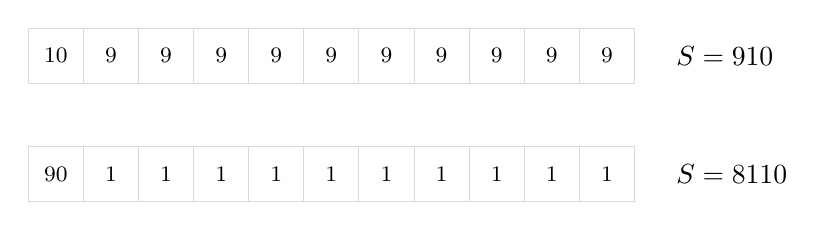
\begin{tikzpicture}[
        node distance=0pt,
        % Stile delle celle: bordo grigio chiaro e font sans-serif
        cell/.style={
            draw=black!15, 
            minimum size=0.7cm, 
            inner sep=0pt, 
            font=\footnotesize
        },
        header/.style={
            anchor=west
        },
        result/.style={
            anchor=west,
            xshift=0.4cm
        }
    ]
        
    \node[cell] (a0) at (0, 0) {10};
    \foreach \i [remember=\i as \last (initially 0)] in {1,...,10} {
        \node[cell] (a\i) at (\i*0.7, 0) {9};
    }
    \node[result] at (a10.east) {$S = 910$};


    \node[cell] (b0) at (0, -1.5) {90};
    \foreach \i [remember=\i as \last (initially 0)] in {1,...,10} {
        \node[cell] (b\i) at (\i*0.7, -1.5) {1};
    }
    \node[result] at (b10.east) {$S = 8110$};

    % --- SCENARIO B: Distribuzione Sbilanciata ---
    % \node[header, font=\small] at (0, -0.8) {Scenario B: Item counts (Skewed)};

    % Prima cella
    % \node[cell] (b1) at (0, -1.5) {90};
    
    % Ciclo per le altre 10 celle (valore 1)
    % \foreach \i [remember=\i as \last (initially 1)] in {2,...,11} {
    %     \node[cell, right=of b\last] (b\i) {1};
    % }

    % Risultato Surprise Number
    % \node[result] at (b11.east) {$S = 8,110$};

    \end{tikzpicture}
    
\end{figure}
\end{example}

Si presenta un metodo di calcolo di momenti su una Stream chiamato \emph{AMS} (\textit{Alon Matias Szegedy}).

\subsubsection{Metodo AMS}
Il metodo \emph{AMS} funziona con tutti i momenti e fornisce una stima \emph{unbiased}, prendendo ad esempio il secondo momento, si procede come segue

\begin{enumerate}
    \item prendi e aggiorna un campione di variabili aleatorie indipendenti $\{X_j \mid j=1,\dots,k\}$
    \item per ogni variabile $X$ viene mantenuto $X.el$ corrispondente a $i \in I$ e $X.val$ corrispondente al conto delle frequenze
\end{enumerate}

Resta ora da definire come impostare $X.val$ e $X.el$
\begin{enumerate}
    \item Input: Stream $I$ di lunghezza $L$
    \item viene scelto un timestamp $t \in_u [1,L]$
    \item di imposta $X.el = i$ con $i = I[t]$
    \item si calcola $X.val = c$ come il numero di $i$ occorrenze nella sotto-Stream $[1,\dots,L]$
    \item Output: la stima per il secondo momento $\sum_{i}{m_i}^2$ 
    \[
        S = f(X) = L \cdot (2 c -1)
    \]
\end{enumerate}
\textit{Nota}: L'algoritmo calcola più $X$ $(X_1,X_2,\dots,X_k)$ la stima sarà data da $S = \frac{1}{k}\sum_{j=1}^{k}f(X_j)$.

Si procede con l'analisi dell'algoritmo
\subsubsection*{Analisi}
Sia $t$ una variabile aleatoria, un elemento $i$, conteggio $c$ e la lunghezza della Stream $L$ come definito dall'algoritmo \textit{AMS}
\begin{align*}    
    \E{L \cdot (2c -1)} &= \sum_{i=1}^{L} L\cdot (c[i] - 1) \frac{1}{L}\\
    &= \boxed{\sum_{i=1}^{L} (2\cdot c[i] - 1)}
\end{align*}
È necessario calcolare l'ultimo risultato per ogni $a \in A$ fissata sia $j_1,\dots,j_{m_a}$ le occorrenze di $a$ nella Stream $I = I[1,\dots,L]$ allora
\[
    c(j_1) = m_a \quad c(j_2) = m_a -1 \quad \dots \quad c(j_{m_a}) = 1
\]
Quindi è possibile riscrivere il risultato ottenuto come $\sum_{a \in A} \sum_{z = 1}^{m_a}(2j -1)$ 
\[
    \sum_{z = 1}^{m_a}(2j -1) = m_{a}^{2}
\] infine 
\[
    \E{L (2c -1)} = \E{S} = \sum_{i=1}m_{i}^{2}
\]
Il secondo momento è dato da $S = \sum_{i} {m_i}^2$. $c_t$ è il numero di occorrenze dell'elemento dal tempo $t$ in poi.
\begin{align*}
    \E{S} &= \frac{1}{n}\sum_{t=1}^{n}n(2c_t - 1) = \\
    &= \frac{1}{n} \sum_{i} n (1 + 3 + \dots, 2m_i - 1)\\
    &= 2\frac{m_i (m_i + 1)}{2} - m_i = m_{i}^2
\end{align*}

Si ottiene
\[
    \E{S= f(X)} = \frac{1}{n}\sum_{i} n(m_i)^2
\]
Ovvero il valore atteso è proprio il secondo momento.

\subsubsection*{Momenti di ordine maggiore}
Come anticipato l'algoritmo \textit{AMS} permette di stimare diversi momenti
\begin{itemize}
    \item per $k = 2$ si ha $n(2c - 1)$
    \item per $k = 3$ si ha $n(3c^2 - 3c +1)$
\end{itemize}
con $c = X.val$.
Per $k = 2$ $(1 + 3 + \dots + 2m_i -1)$ e la somma dei termini $2c - 1$ fa $m^2$.
\noindent

Per $k = 3$ $c^3 - (c-1)^3 = 3c^2 - 3c +1$, si presenta una generalizzazione per $k$, in cui la stima è $n(c^k - (c-1)^k)$

\subsubsection*{Combinazione dei Sample}
Nella pratica vengono mantenute tante variabili indipendenti $X$ per quante possono essere mantenute in memoria, si dividono in gruppi in cui si fa la media, e si prende la mediana.

\vspace{1em}\noindent
Per una Stream di lunghezza $L$ \emph{molto grande} o \emph{infinita}
% pag 47 ch04 8 12